\section{Hand Assembly}

This section contains illustrated instructions for assembling all remaining hand components and for attaching them on the palm. For each assembly step, a table listing all necessary parts and tools/materials will be provided for convenience.

\subsection{Attaching the Fingers on the Palm}

%The necessary parts and tools to attach all fingers on the palm are listed in table \ref{fingerspalmattachment}, while Fig. 7.1.1 demonstrates the assembly.

\begin{table}[ht!]
	\centering
	\begin{tabular}{ | c | c | c |}
		\hline
		\multicolumn{3}{|c|}{{\textbf{Parts List 7.1.1}}} \\ \hline		
		{\bf{No}} & {\bf{Part Name}} & {\bf{Qty}}\\ \hline
    		1 & index & 1  \\ \hline
    		2 & middle & 1  \\ \hline
		3 & ring & 1 \\ \hline
		4 & pinky & 1 \\ \hline
		5 & palmUp & 1 \\ \hline
		\multicolumn{3}{|c|}{{\textbf{Tools}}} \\ \hline
		\multicolumn{3}{|c|}{{{Long Needles}}} \\ \hline
		\multicolumn{3}{|c|}{{{Nylon Fishing Line}}} \\ \hline
		\multicolumn{3}{|c|}{{{Cutter}}} \\ \hline
		\multicolumn{3}{|c|}{{{Long-Nose Pliers with Side-Cutting}}} \\ \hline
		\multicolumn{3}{|c|}{{{Scissors}}} \\ \hline
		
    	\end{tabular}
\end{table}

\vspace{0.5cm}

\begin{center}
\begin{tikzpicture}
\node [mybox] (box){%

  	\begin{minipage}[b]{0.45\linewidth}\centering
	\begin{tabular}{ c }
		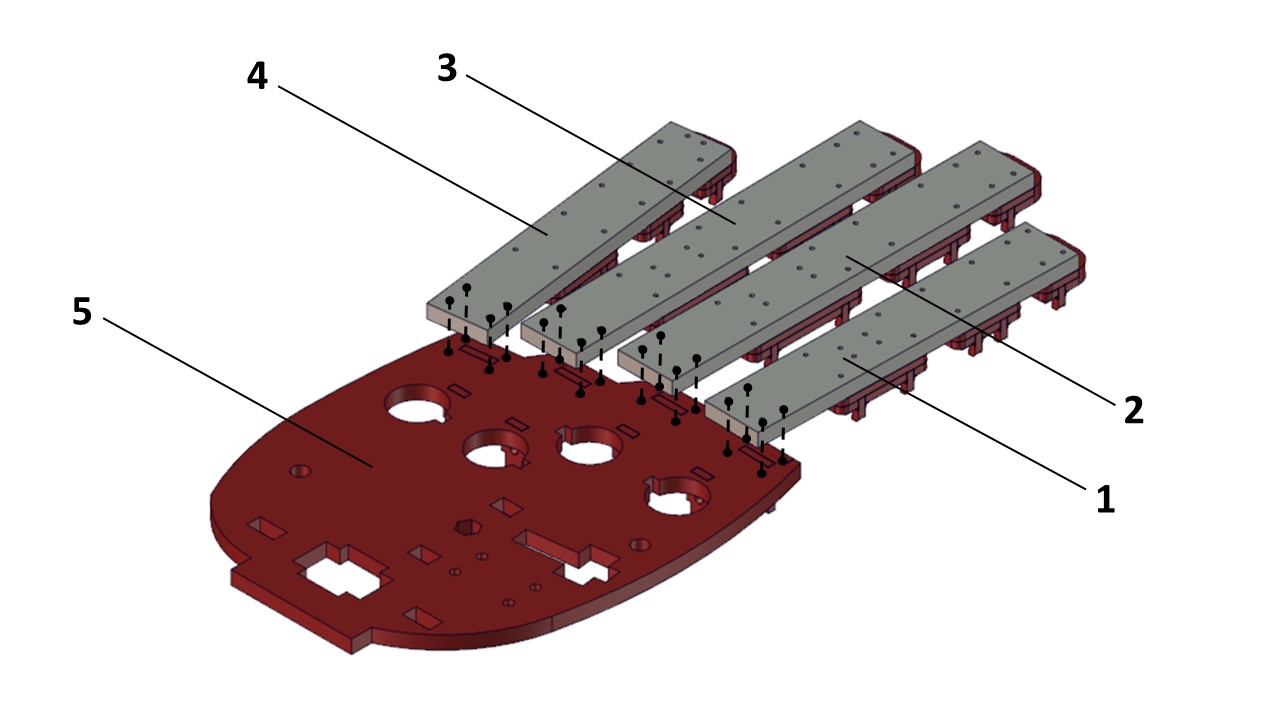
\includegraphics[width = 8cm]{figures/Hand/palmUp_fingers_re.jpg}
    	\end{tabular}
	\end{minipage}
	
	\hspace{1.0cm}	
	
	\begin{minipage}[b]{0.4\linewidth}\centering
	\begin{tabular}{  l  l }
		{\circled{1}} & {Stitch fingers parts 1-4}\\
		{} & {on the palm following}\\
		{} &  {the procedure described}\\
		{} & {in steps 6.2.5 - 6.2.7.}\\
	\end{tabular}
  	\end{minipage}
	};
\node[mytitle, right=10pt] at (box.north west) {Board 7.1.1: Attaching the Fingers on the Palm};
\end{tikzpicture}%
\end{center}

\newpage

\subsection{Building/Attaching the Locking Buttons on the Palm}



\begin{table}[ht!]
	\centering
  	%\begin{minipage}[b]{0.50\linewidth}\centering
	\scalebox{0.97}{
	\begin{tabular}{ | c | c | c |}
		\hline
		\multicolumn{3}{|c|}{{\textbf{Parts List 7.2.1}}} \\ \hline
		{\bf{No}} & {\bf{Part Name}} & {\bf{Qty}}\\ \hline
     	1 & palmUp & 1  \\ \hline
		2 & buttonBase & 4 \\ \hline
		\multicolumn{3}{|c|}{{\bf{Material}}} \\ \hline
		\multicolumn{3}{|c|}{{{ABS Glue}}} \\ \hline
	\end{tabular}
	}
	%\caption{The Parts required to build the button bases on the Palm along with the glue type.}
	%\label{buttonspalm}
\end{table}

\begin{center}
\begin{tikzpicture}
\node [mybox] (box){%
  	\begin{minipage}[b]{0.50\linewidth}\centering
	\begin{tabular}{ l }
           	     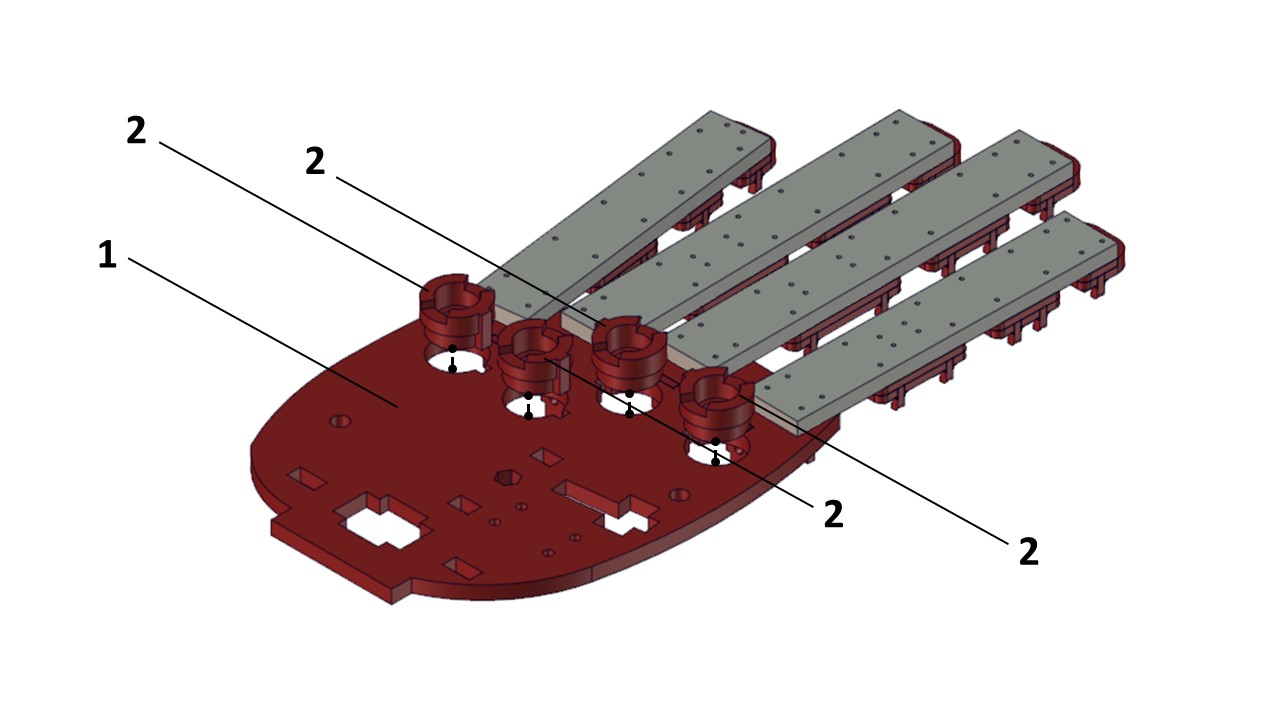
\includegraphics[trim={2cm, 1cm, 4cm, 1cm}, clip,scale = 0.25]{figures/Hand/palmUpFingers_buttonBase_re.jpg} 
    	\end{tabular}
	\end{minipage}
	\begin{minipage}[b]{0.4\linewidth}
	\begin{tabular}{  l  l }
		{\circled{1}} & {Glue the buttonBase parts}\\
		{} & {on the palmUp part in the}\\
		{} & {designated positions.}\\
    	\end{tabular}
  	\end{minipage}
};
\node[mytitle, right=10pt] at (box.north west) {Board 7.2.1: Attaching the Button Bases on the Palm};
\end{tikzpicture}%
\end{center}


\begin{table}[ht!]
\centering
	\scalebox{0.97}{
	\begin{tabular}{ | c | c | c |}
		\hline
		\multicolumn{3}{|c|}{{\bf{Parts List 7.2.2}}}\\ \hline
		{\bf{No}} & {\bf{Part Name}} & {\bf{Qty}}\\ \hline
    		1 & buttonAxle & 4  \\ \hline
   		2 & buttonFrame & 4  \\ \hline
        3 & M2X16 Dowel Pin & 4 \\ \hline
		4 & Compression Spring 6mm L, & 4 \\  & 9mm OD, 1mm WD  & \\ \hline
		5 & Structure of Board 7.2.1 & 1 \\ \hline
 		\multicolumn{3}{|c|}{{\bf{Tools/Materials}}} \\ \hline
 		\multicolumn{3}{|c|}{{{ABS Glue}}} \\ \hline
 		\multicolumn{3}{|c|}{{{Long-Nose Pilers with Side-Cutting}}} \\ \hline		
    	\end{tabular}
	}
\end{table}

\begin{center}
\begin{tikzpicture}
\node [mybox] (box){%
	\begin{minipage}[b]{0.50\linewidth}
	\begin{tabular}{ l }
 	 	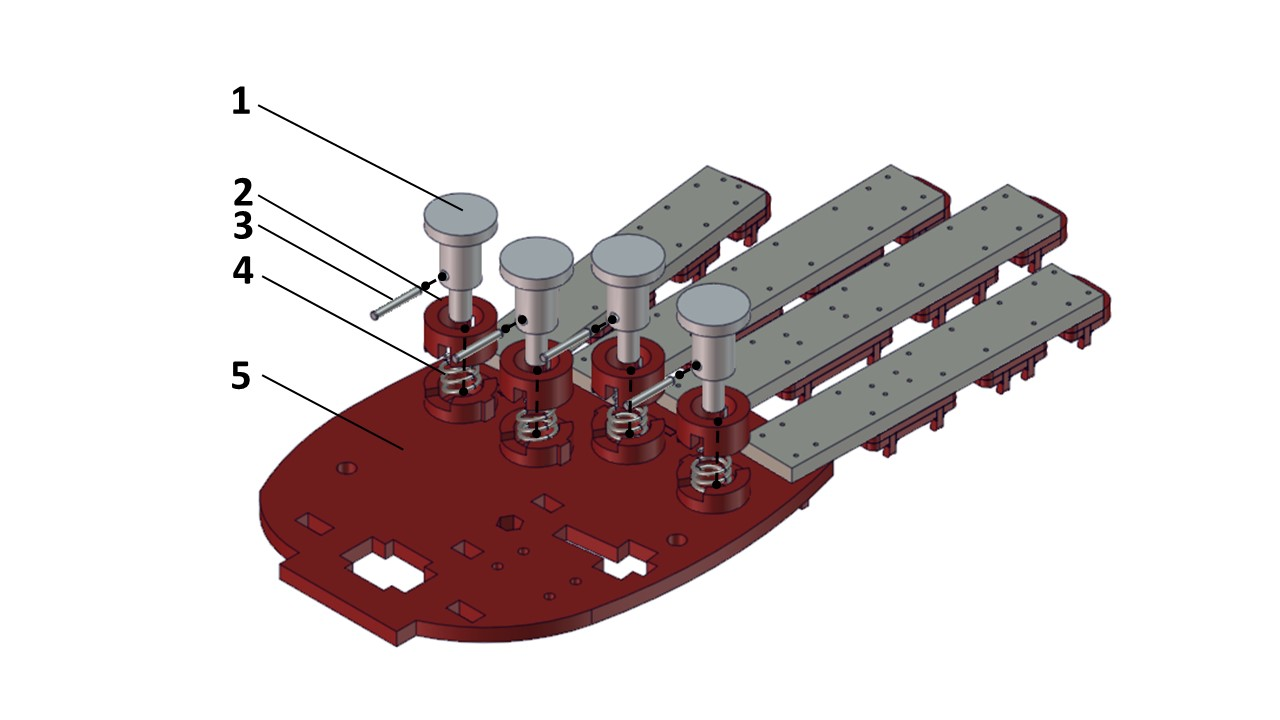
\includegraphics[trim={6cm, 1cm, 1cm, 1cm}, clip,scale = 0.3]{figures/Hand/palmUpFingersButtonBase_restButton_re.jpg} 
    	\end{tabular}
  	\end{minipage}
  	\begin{minipage}[b]{0.50\linewidth}\centering
	\begin{tabular}{ l l}
		{\circled{1}} & {Glue the buttonFrame parts}\\
		{} & {on the buttonBase's (see Parts List/}\\
		{} & {Board 7.2.1).} \\ \\
		{\circled{2}} & {Insert the compression springs in}\\
		{} & {the buttonFrame slots.} \\ \\
		{\circled{3}} & {Insert the buttonAxle parts in the}\\
		{} & {buttonFrame slots.} \\ \\
		{\circled{4}} & {Insert the M2X16 pins in the}\\
		{} & {buttonAxle slots.} \\            
		%parts, as you pushing it \\ downwards.	
    	\end{tabular}
	\end{minipage}
};
\node[mytitle, right=10pt] at (box.north west) {Board 7.2.2: Building/Fixing the Buttons on the Palm};
\end{tikzpicture}%
\end{center}

\newpage

\subsection{Building the Thumb Locking Mechanism}

\begin{table}[ht]
\centering
	\scalebox{0.97}{
	\begin{tabular}{ |c | c | c |}
		\hline
 		\multicolumn{3}{|c|}{{\bf{Parts List 7.3.1}}} \\ \hline		
		{\bf{No}} & {\bf{Part Name}} & {\bf{Qty}}\\ \hline
    		1 & toothedMechanism & 1  \\ \hline
    		2 & palmDown & 1  \\ \hline
 		\multicolumn{3}{|c|}{{\bf{Tools}}} \\ \hline
 		\multicolumn{3}{|c|}{{{ABS Glue}}} \\ \hline
    	\end{tabular}
	}
\end{table}


\begin{center}
\begin{tikzpicture}
\node [mybox] (box){%
  	\begin{minipage}[b]{0.50\linewidth}\centering
	\begin{tabular}{ c }
		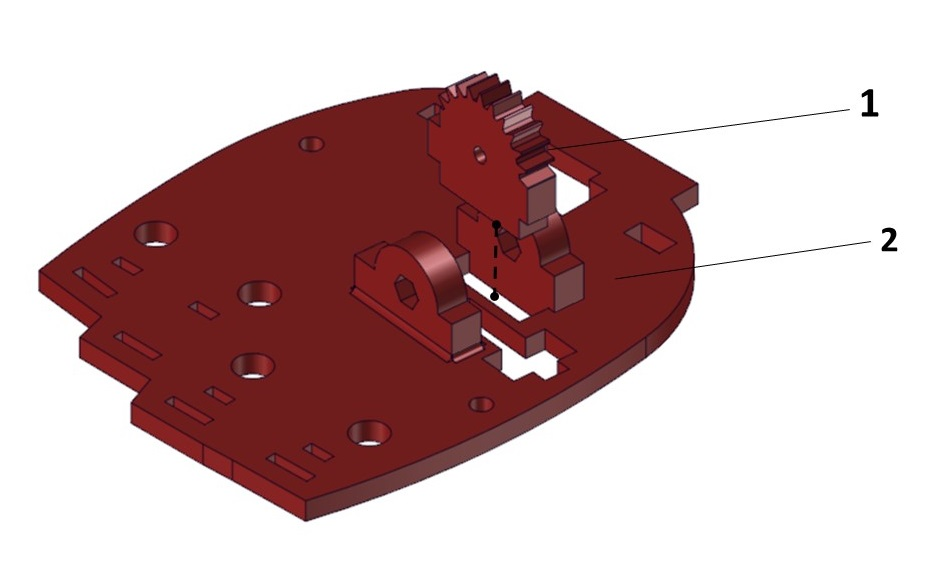
\includegraphics[trim={1cm, 1cm, 1cm, 1cm}, clip,scale = 0.32]{figures/Hand/palmDown_toothedMechanism_re.jpg}
    	\end{tabular}
	\end{minipage}
	\begin{minipage}[b]{0.35\linewidth}
	\begin{tabular}{ l l}
		{\circled{1}} & {Glue the toothedMechanism}\\
		{} & {on the palmDown part.}
    	\end{tabular}
  	\end{minipage}
};
\node[mytitle, right=10pt] at (box.north west) {Board 7.3.1: Fixing the toothedMechanism on the Palm};
\end{tikzpicture}%
\end{center}

\begin{table}[h]
\centering
	\scalebox{0.97}{
	\begin{tabular}{ |c | c | c |}
		\hline
 		\multicolumn{3}{|c|}{{\bf{Parts List 7.3.2}}} \\ \hline	
		{\bf{No}} & {\bf{Part Name}} & {\bf{Qty}}\\ \hline
    		1 & lockMechanismBracket & 2  \\ \hline
    		2 & lockMechanismSupport & 1  \\ \hline
 		\multicolumn{3}{|c|}{{\bf{Material}}} \\ \hline
 		\multicolumn{3}{|c|}{{ABS Glue}} \\ \hline
    	\end{tabular}
	}
\end{table}


\begin{center}
\begin{tikzpicture}
\node [mybox] (box){%
  	\begin{minipage}[b]{0.4\linewidth}\centering
	\begin{tabular}{ l }
		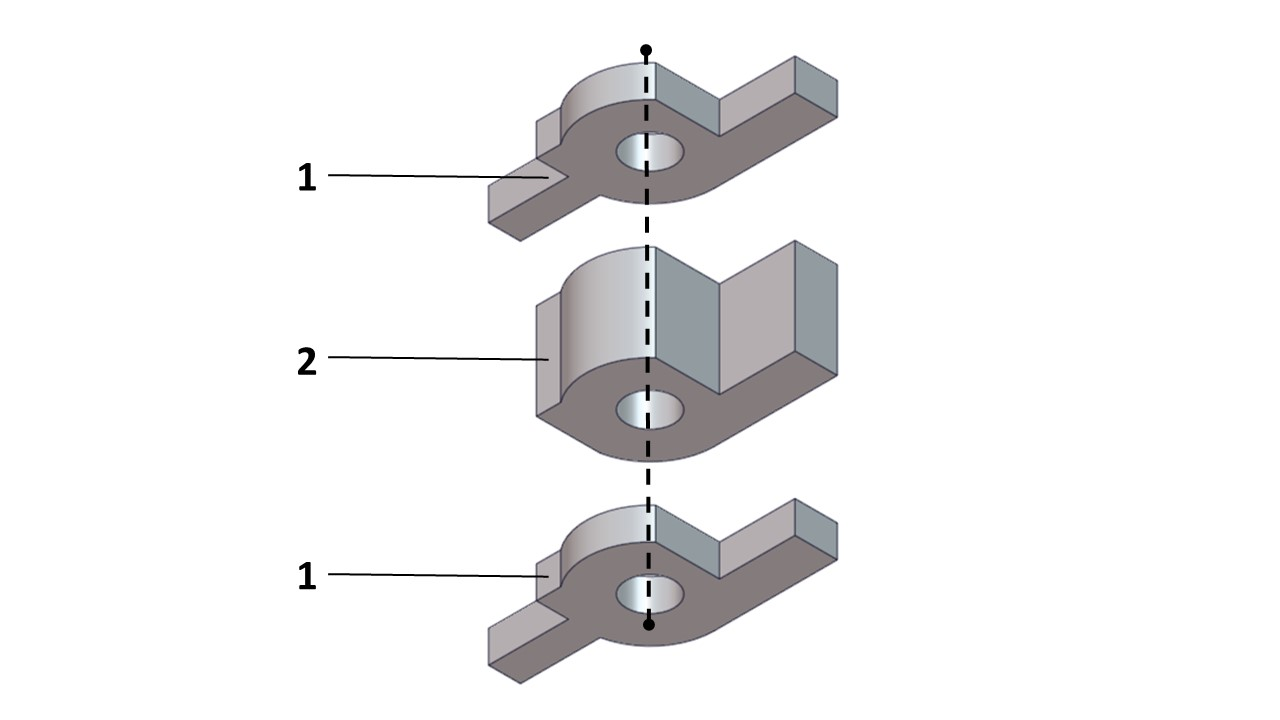
\includegraphics[trim={8cm, 1cm, 1cm, 0cm}, clip,scale = 0.25]{figures/Hand/lockingMechanismPreAssembled1.jpg}
    	\end{tabular}
	\end{minipage}
	\begin{minipage}[b]{0.5\linewidth}
	\begin{tabular}{ l l }
		{\circled{1}} & {Align the lockMechanismBracket parts}\\
		{} & {with the lockMechanismSupport part.} \\ \\
		{\circled{2}} & {Glue the parts.} \\
    	\end{tabular}
  	\end{minipage}
};
\node[mytitle, right=10pt] at (box.north west) {Board 7.3.2: Building the Thumb Locking Mechanism I};
\end{tikzpicture}%
\end{center}

\newpage

\begin{table}[ht!]
\centering
	\scalebox{0.97}{
	\begin{tabular}{ |c | c | c |}
		\hline
 		\multicolumn{3}{|c|}{{\bf{Parts List 7.3.3}}} \\ \hline	
		{\bf{No}} & {\bf{Part Name}} & {\bf{Qty}}\\ \hline
		1 & Structure of Board 7.3.2 & 1  \\ \hline
		2 & toothedBlockMechanism & 1  \\ \hline
    		3 & thumbButton & 1  \\ \hline   		
 		\multicolumn{3}{|c|}{{\bf{Material}}} \\ \hline
 		\multicolumn{3}{|c|}{{ABS Glue}} \\ \hline
    	\end{tabular}
	}
\end{table}


\begin{center}
\begin{tikzpicture}
\node [mybox] (box){%
  	\begin{minipage}[b]{0.48\linewidth}\centering
	\begin{tabular}{ l }
		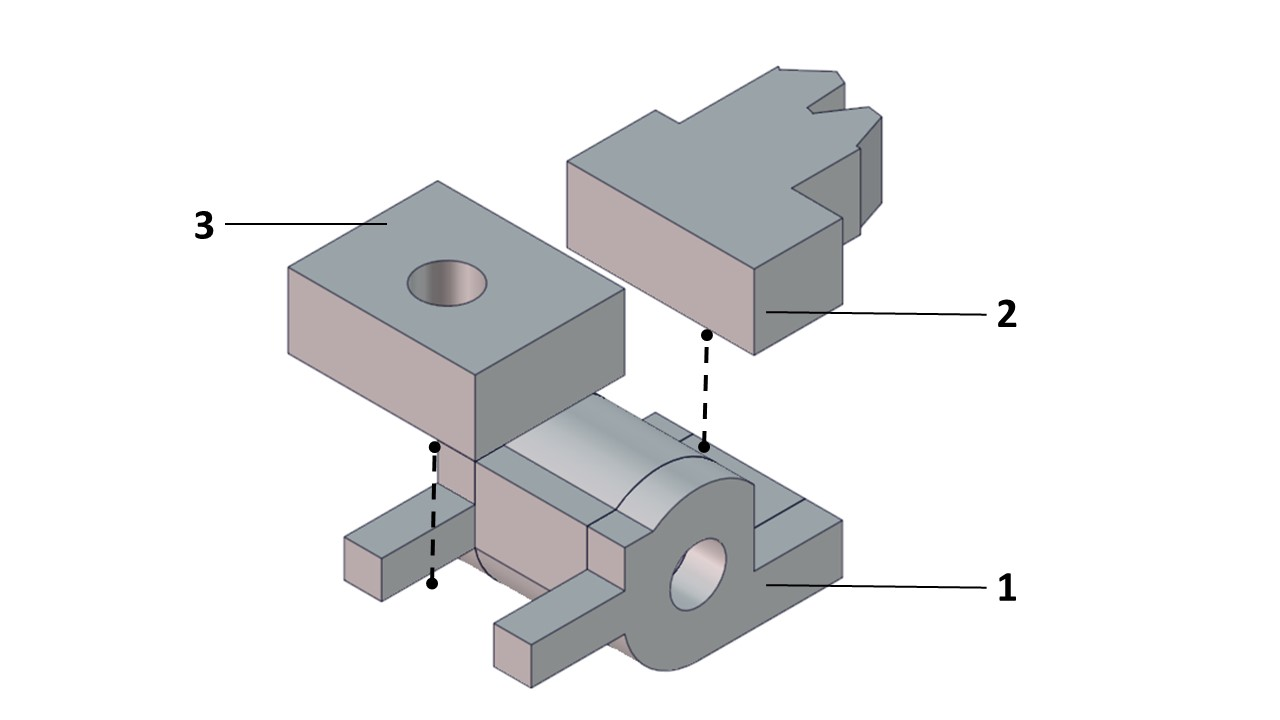
\includegraphics[trim={4cm, 0cm, 1cm, 0cm}, clip,scale = 0.25]{figures/Hand/lockingMechanismPreAssembled2.jpg}
    	\end{tabular}
	\end{minipage}
	\begin{minipage}[b]{0.5\linewidth}
	\begin{tabular}{ l l }
		{\circled{1}} & {Glue the thumbButton and the}\\
		{} & {toothedBlockMechanism parts}\\
		{} & {with the Structure of Board 7.3.2.}\\
    	\end{tabular}
  	\end{minipage}
};
\node[mytitle, right=10pt] at (box.north west) {Board 7.3.3: Building the Thumb Locking Mechanism II};
\end{tikzpicture}%
\end{center}


\begin{table}[ht!]
\centering
	\scalebox{0.97}{
	\begin{tabular}{ |c | c | c |}
		\hline
 		\multicolumn{3}{|c|}{{\bf{Parts List 7.3.4}}} \\ \hline		
		{\bf{No}} & {\bf{Part}} & {\bf{Qty}}\\ \hline
		1 & Strucutre of Board 7.3.3 & 1  \\ \hline
		2 & M3 Nut & 1  \\ \hline
		3 & M3 Washer & 1  \\ \hline
    		4 & M3X6 Socket Cup Screw & 1  \\ \hline
 		\multicolumn{3}{|c|}{{\bf{Tools}}} \\ \hline
		\multicolumn{3}{|c|}{{Allen Wrench}}\\ \hline		
    	\end{tabular}
	}
\end{table}


\begin{center}
\begin{tikzpicture}
\node [mybox] (box){%
  	\begin{minipage}[b]{0.50\linewidth}\centering
	\begin{tabular}{ l }
		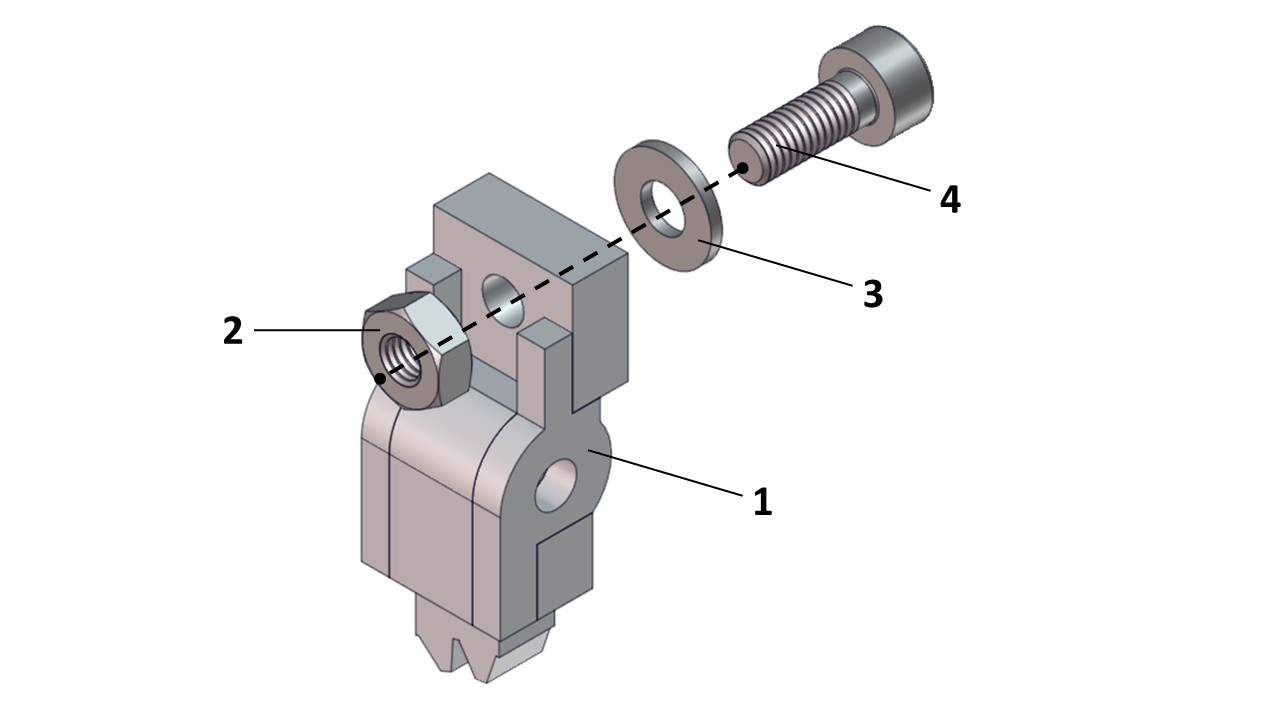
\includegraphics[trim={5cm, 0cm, 1cm, 0cm}, clip,scale = 0.3]{figures/Hand/thumbMovingMechansim_lockingMechanism1.jpg}
    	\end{tabular}
	\end{minipage}
	\begin{minipage}[b]{0.5\linewidth}
	\begin{tabular}{ l l }
		{\circled{1}} & {Align the fasteners with the}\\
		{} &  {Structure of Board 7.3.3.} \\ \\
		{\circled{2}} & {Screw the M3X6 bolt through}\\
		{} & {all fasteners.} \\
    	\end{tabular}
  	\end{minipage}
};
\node[mytitle, right=8pt] at (box.north west) {Board 7.3.4: Building the Thumb Locking Mechanism III};
\end{tikzpicture}%
\end{center}


\begin{table}[ht!]
\centering
	\scalebox{0.97}{
	\begin{tabular}{ |c | c | c |}
		\hline
 		\multicolumn{3}{|c|}{{\bf{Parts List 7.3.5}}} \\ \hline		
		{\bf{No}} & {\bf{Part}} & {\bf{Qty}}\\ \hline
		1 & thumbMovingMechanism part & 1  \\ \hline
		2 & M3X18 Set Screw & 1  \\ \hline
		3 & M3 Nut & 2  \\ \hline
		4 & Structure of Board 7.3.4 & 1  \\ \hline
    		5 & Compression Spring 3mm L, & 1 \\  & 3.5mm OD, 0.5mm WD & \\ \hline
 		\multicolumn{3}{|c|}{{\bf{Tools}}} \\ \hline
		\multicolumn{3}{|c|}{{Screwdriver}}\\ \hline
    	\end{tabular}
	}
\end{table}


\begin{center}
\begin{tikzpicture}
\node [mybox] (box){%
  	\begin{minipage}[b]{0.38\linewidth}\centering
	\begin{tabular}{ l }
		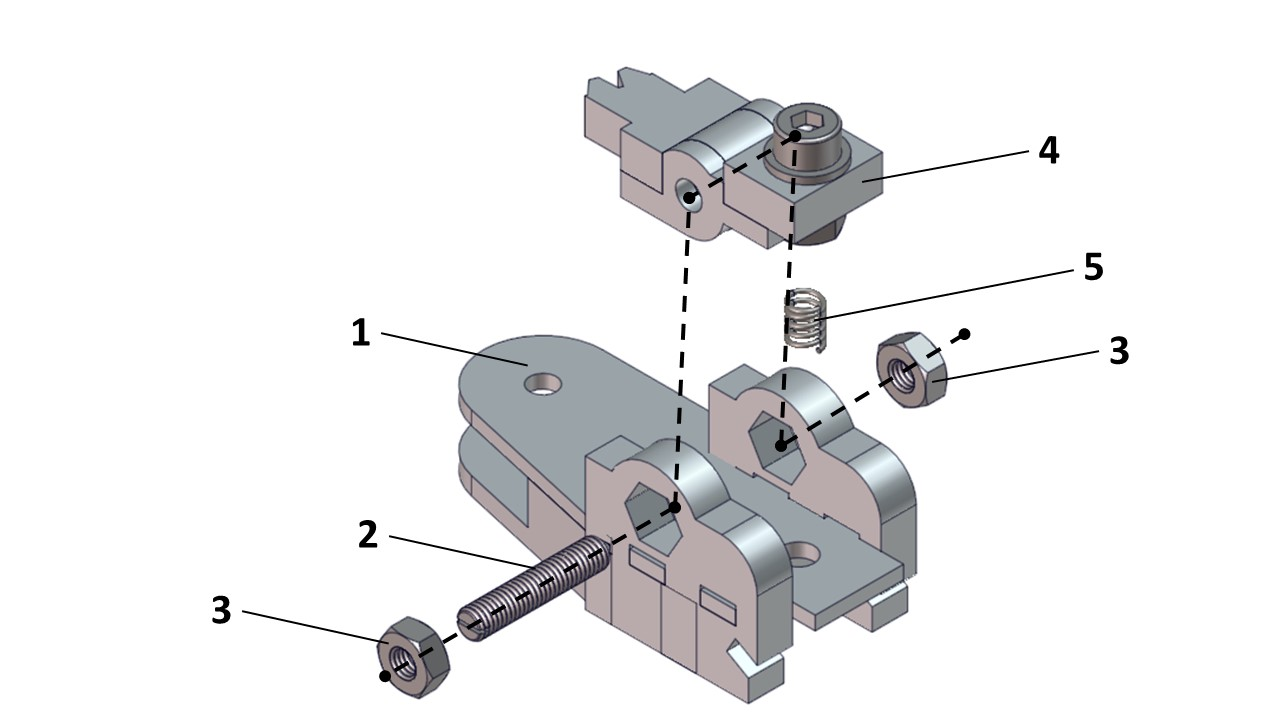
\includegraphics[trim={5cm, 0cm, 1cm, 0cm}, clip,scale = 0.22]{figures/Hand/thumbMovingMechansim_lockingMechanism2.jpg}
    	\end{tabular}
	\end{minipage}
	\begin{minipage}[b]{0.5\linewidth}
	\begin{tabular}{ l l }
	    {\circled{1}} & {Align the compression spring with the}\\
	    {} & {Structure of Board 7.3.4 as shown.} \\ \\
		{\circled{2}} & {Align the two M3 nuts with the sockets of}\\
		{} & {the thumbMovingMechanism part.} \\ \\
		{\circled{3}} & {Screw the M3X18 Set Screw}\\
		{} & {through all fasteners.} \\ \\
    	\end{tabular}
  	\end{minipage}
};
\node[mytitle, right=10pt] at (box.north west) {Board 7.3.5: Building the Thumb Locking Mechanism IV};
\end{tikzpicture}%
\end{center}


\begin{table}[ht!]
\centering
	\scalebox{0.97}{
	\begin{tabular}{ |c | c | c |}
		\hline
 		\multicolumn{3}{|c|}{{\bf{Parts List 7.3.6}}} \\ \hline				
		{\bf{No}} & {\bf{Part}} & {\bf{Qty}}\\ \hline
    		1 & thumb & 1  \\ \hline
    		2 & Structure of Board 7.3.5 & 1  \\ \hline
 		\multicolumn{3}{|c|}{{\bf{Tools}}} \\ \hline
 		\multicolumn{3}{|c|}{{ABS Glue}} \\ \hline
    	\end{tabular}
	}
\end{table}

\begin{center}
\begin{tikzpicture}
\node [mybox] (box){%
  	\begin{minipage}[b]{0.50\linewidth}\centering
	\begin{tabular}{ c }
		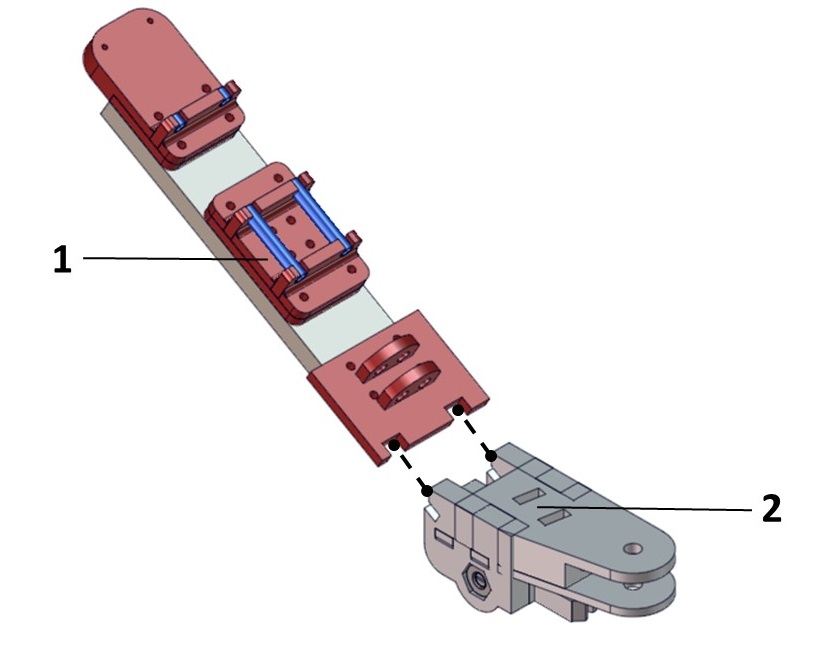
\includegraphics[trim={0cm, 0cm, 1cm, 0cm}, clip,scale = 0.4]{figures/Hand/thumbMovingMechansimLockingMechanism_thumb.jpg}
    	\end{tabular}
	\end{minipage}
	\begin{minipage}[b]{0.5\linewidth}
	\begin{tabular}{ l l}
		{\circled{1}} & {Center the thumb part.} \\ \\
		{\circled{2}} & {Glue the thumb with the}\\
		{} & {Structure of Board 7.3.5.}\\
    	\end{tabular}
  	\end{minipage}
};
\node[mytitle, right=10pt] at (box.north west) {Board 7.3.6: Attaching the Thumb on the Thumb Locking Mechanism};
\end{tikzpicture}%
\end{center}

\newpage 

\subsection{Tendon Routing System/Servo Base Assembly \& Mount On the Palm}

\begin{table}[ht!]
\centering
	\scalebox{0.9}{
	\begin{tabular}{ |c | c | c |}
		\hline
		\multicolumn{3}{|c|}{{\textbf{Parts List 7.4.1}}}\\ \hline
		{\bf{No}} & {\bf{Part Name}} & {\bf{Qty}}\\ \hline
    		1 & M3 Nut & 2  \\ \hline
    		2 & M3X12 Set Screw & 1  \\ \hline
    		3 & basePulleyInsidePalm & 2  \\ \hline
    		4 & M3 Washer & 2  \\ \hline
    		5 & V-Grooved Sealed Ball Bearing & 1  \\ \hline
 		\multicolumn{3}{|c|}{{\bf{Tools}}} \\ \hline
		\multicolumn{3}{|c|}{{Long-Nose Pilers with Side-Cutting}}\\ \hline
		\multicolumn{3}{|c|}{{Screwdriver}}\\ \hline
    	\end{tabular}
	}
\end{table}

\begin{center}
\begin{tikzpicture}
\node [mybox] (box){%
  	\begin{minipage}[b]{0.5\linewidth}\centering
	\begin{tabular}{ l }
		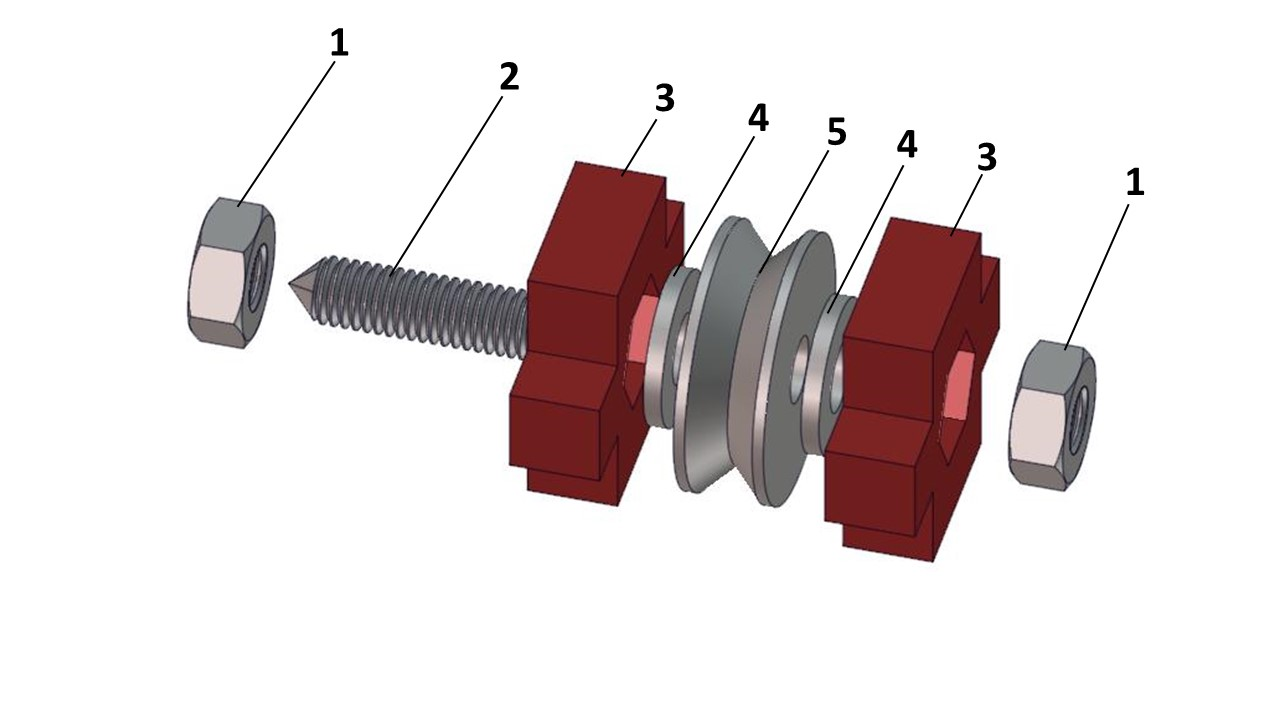
\includegraphics[trim={5cm, 4.2cm, 1cm, 0cm}, clip,scale = 0.23]{figures/Hand/pulleyInsidePalm_re.jpg}
    	\end{tabular}
	\end{minipage}
	\begin{minipage}[b]{0.5\linewidth}
	\begin{tabular}{ l l }
		{\circled{1}} & {Align the two M3 nuts with the sockets of}\\
		{} & {basePulleyInsidePalm parts.} \\ \\
		{\circled{2}} & {Align the M3 Nuts, M3 Washers and pulley}\\
		{} & {as shown.} \\ \\
		{\circled{3}} & {Screw the M3X12 Set Screw through}\\
		{} & {all fasteners.} \\
    	\end{tabular}
  	\end{minipage}
};
\node[mytitle, right=10pt] at (box.north west) {Board 7.4.1: Building the Tendon Routing Pulley Base I};
\end{tikzpicture}%
\end{center}


\begin{table}[ht!]
\centering
	\scalebox{0.9}{
	\begin{tabular}{ |c | c | c |}
		\hline
 		\multicolumn{3}{|c|}{{\textbf{Parts List 7.4.2}}} \\ \hline		
		{\bf{No}} & {\bf{Part Name}} & {\bf{Qty}}\\ \hline
    		1 & M3 Nut & 1  \\ \hline
    		2 & M3 Washer & 2  \\ \hline
    		3 & V-Grooved Sealed Ball Bearing & 1  \\ \hline
    		4 & supportPulleyPalmUpAssem & 1  \\ \hline
    		5 & M3X10 Socket Cup Screw & 1  \\ \hline
 		\multicolumn{3}{|c|}{{\bf{Tools}}} \\ \hline
 		\multicolumn{3}{|c|}{{{Long-Nose Pilers with Side-Cutting}}} \\ \hline
 		\multicolumn{3}{|c|}{{{Allen Wrench}}} \\ \hline
    	\end{tabular}
	}
\end{table}

\begin{center}
\begin{tikzpicture}
\node [mybox] (box){%
  	\begin{minipage}[b]{0.50\linewidth}\centering
	\begin{tabular}{ l }
		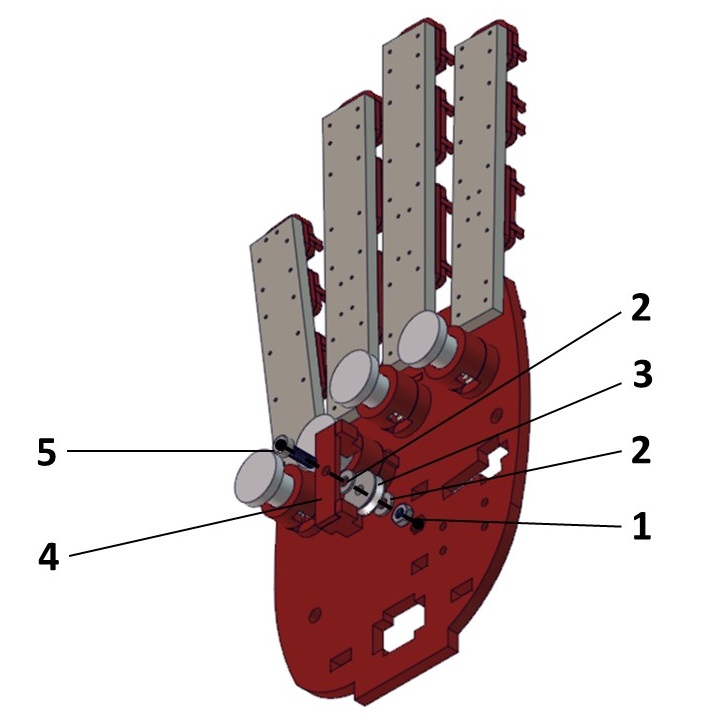
\includegraphics[trim={0cm, 0cm, 1cm, 0cm}, clip,scale = 0.38]{figures/Hand/palmUp_fingers_buttons_upPulley.jpg}
    	\end{tabular}
	\end{minipage}
	\begin{minipage}[b]{0.5\linewidth}
	\begin{tabular}{ l l }
		{\circled{1}} & {Align the M3 nut with the socket}\\
		{} & {of the structure of Board 7.2.2.} \\ \\
		{\circled{2}} & {Align the M3 Washers,}\\
		{} &  {the supportPulleyPalmUpAssem part}\\
		{} & {and the pulley as shown.} \\ \\
		{\circled{3}} & {Screw the M3X6 bolt through}\\
		{} &  {all fasteners.} \\
    	\end{tabular}
  	\end{minipage}
};
\node[mytitle, right=10pt] at (box.north west) {Board 7.4.2: Building the Support of the Pulley Base};
\end{tikzpicture}%
\end{center}


\begin{table}[ht!]
\centering
	\scalebox{0.97}{
	\begin{tabular}{ |c | c | c |}
		\hline
 		\multicolumn{3}{|c|}{{\bf{Parts List 7.4.3}}} \\ \hline		
		{\bf{No}} & {\bf{Part Name}} & {\bf{Qty}}\\ \hline
    		1 & Structure of Board 7.4.2 & 1  \\ \hline
    		2 & M2X10 Machine Screw & 4  \\ \hline
    		3 & Plastic Spacer 4mm & 4  \\ \hline
    		4 & baseHerkulex part & 1  \\ \hline
    		5 & M2 Nut & 4  \\ \hline
 		\multicolumn{3}{|c|}{{\bf{Tools}}} \\ \hline
 		\multicolumn{3}{|c|}{{{Screwdriver}}} \\ \hline
    	\end{tabular}
	}
\end{table}

\begin{center}
\begin{tikzpicture}
\node [mybox] (box){%
  	\begin{minipage}[b]{0.45\linewidth}\centering
	\begin{tabular}{ l }
		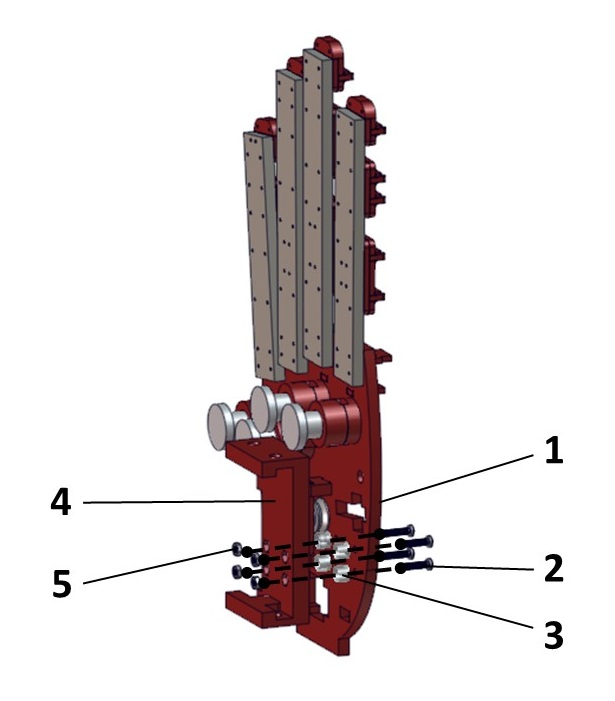
\includegraphics[trim={1cm, 0cm, 1cm, 0cm}, clip,scale = 0.37]{figures/Hand/palmUp_fingers_buttons_upPulley_servoBase.jpg}
    	\end{tabular}
	\end{minipage}
	\begin{minipage}[b]{0.5\linewidth}
	\begin{tabular}{ l l }
		{\circled{1}} & {Align the four M2 nuts with}\\
		{} &  {the baseHerkulex part.} \\ \\
		{\circled{2}} & {Align the baseHerkulex part,}\\
		{} & {the spacer and the M2X10 bolts}\\
		{} & {as shown.} \\ \\
		{\circled{3}} & {Screw the four M2X10 bolts through}\\
		{} & {all fasteners.} \\
    	\end{tabular}
  	\end{minipage}
};
\node[mytitle, right=10pt] at (box.north west) {Board 7.4.3: Building the Support for the Servo Base};
\end{tikzpicture}%
\end{center}

 
\begin{table}[ht!]
\centering
	\scalebox{0.97}{
	\begin{tabular}{ |c | c | c |}
		\hline
 		\multicolumn{3}{|c|}{{\bf{Parts List 7.4.4}}} \\ \hline		
		{\bf{No}} & {\bf{Part Name}} & {\bf{Qty}}\\ \hline
    		1 & low fricion tubes & --  \\ \hline
    		2 & Dyneema & --  \\ \hline
    		3 & barIndexMiddle & 1  \\ \hline
    		4 & barRingPinky & 1  \\ \hline
    		5 & mainBar & 1  \\ \hline
    		6 & Structure of Board 7.4.3 & 1  \\ \hline
 		\multicolumn{3}{|c|}{{\bf{Tools}}} \\ \hline
 		\multicolumn{3}{|c|}{{{Long Needles}}} \\ \hline
 		\multicolumn{3}{|c|}{{{Scissors}}} \\	 \hline				
    	\end{tabular}
	}
\end{table}

\begin{center}
\begin{tikzpicture}
\node [mybox] (box){%
  	\begin{minipage}[b]{0.50\linewidth}\centering
	\begin{tabular}{ c }
		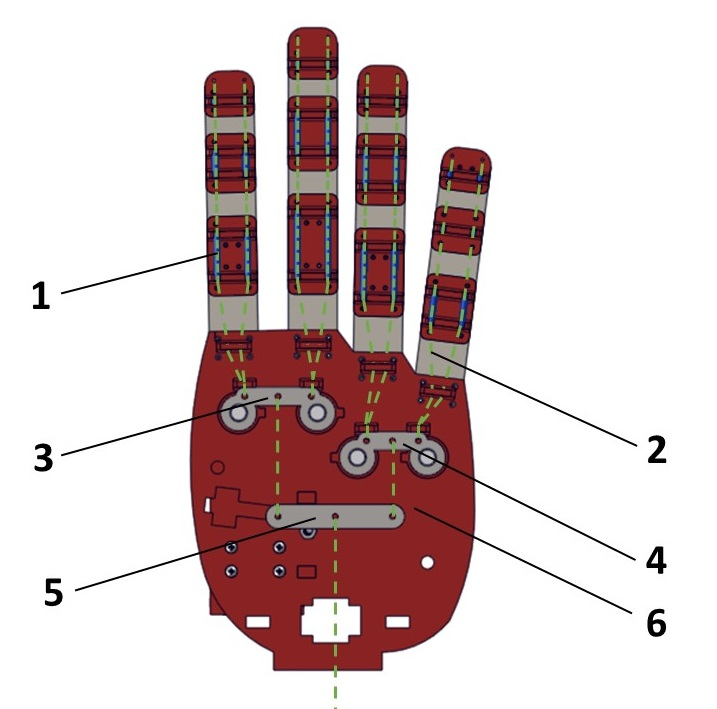
\includegraphics[trim={0cm, 0cm, 1cm, 0cm}, clip,scale = 0.4]{figures/Hand/palmUpComplete_Whiffletree.jpg}
    	\end{tabular}
	\end{minipage}
	\begin{minipage}[b]{0.5\linewidth}
	\begin{tabular}{ l l }
		{\circled{1}} & {Tie the Index and Middle Tendons}\\
		{} & {on the barIndexMiddle part.} \\ \\
		{\circled{2}} & {Tie the Ring and Pinky Tendons}\\
		{} & {on the barRingPinky part.} \\ \\
		{\circled{3}} & {Connect the barRingPinky}\\
		{} & {and barIndexMiddle tendons}\\
		{} & {with the mainBar part as shown.} \\
    	\end{tabular}
  	\end{minipage}
};
\node[mytitle, right=10pt] at (box.north west) {Board 7.4.4: Connecting the Whiffletree Bars with the Dyneema Tendons};
\end{tikzpicture}%
\end{center}


\begin{table}[ht!]
\centering
  	\begin{minipage}[b]{0.50\linewidth}\centering
	\scalebox{0.97}{
	\begin{tabular}{ |c | c | c |}
		\hline
 		\multicolumn{3}{|c|}{{\bf{Parts List 7.4.5}}} \\ \hline				
		{\bf{No}} & {\bf{Part}} & {\bf{Qty}}\\ \hline
    		1 & M3 nut & 1  \\ \hline
    		2 & basePulleyInsidePalm & 2  \\ \hline
    	\end{tabular}
	}
	\end{minipage}
	\hspace{0.5cm}	
\end{table}

\begin{center}
\begin{tikzpicture}
\node [mybox] (box){%
  	\begin{minipage}[b]{0.5\linewidth}\centering
	\begin{tabular}{ l }
		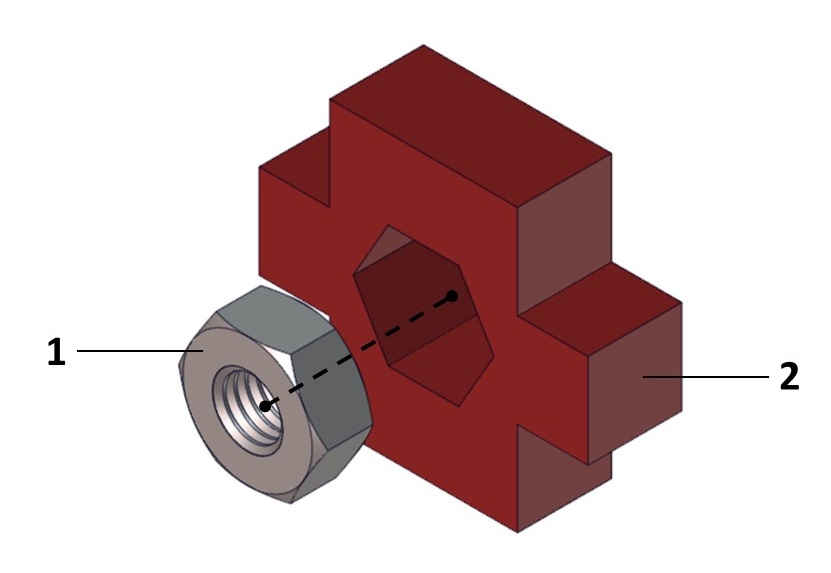
\includegraphics[trim={1cm, 0cm, 0cm, 0cm}, clip,scale = 0.3]{figures/Hand/fastenFlange.jpg}
    	\end{tabular}
	\end{minipage}
	\begin{minipage}[b]{0.5\linewidth}
	\begin{tabular}{ l  l }
		{\circled{1}} & {Place the M3 nut in the socket}\\
		{} & {of basePulleyInsidePalm part.} \\ \\
		{\circled{2}} & {Repeat step \circled{1} for a second part.} \\
    	\end{tabular}
  	\end{minipage}
};
\node[mytitle, right=10pt] at (box.north west) {Board 7.4.5: Building the Support of the Pulley Base II};
\end{tikzpicture}%
\end{center}

\begin{table}[ht!]
\centering
  	\begin{minipage}[b]{0.50\linewidth}\centering
	\scalebox{0.97}{
	\begin{tabular}{ |c | c | c |}
		\hline
	 	\multicolumn{3}{|c|}{{\bf{Parts List 7.4.6}}} \\ \hline			
		{\bf{No}} & {\bf{Part}} & {\bf{Qty}}\\ \hline
    		1 & Structure of Board 7.4.1 & 1  \\ \hline
    		2 & Structure of Board 7.4.4 & 1  \\ \hline
    		3 & Structure of Board 7.4.5 & 2  \\ \hline
    	\end{tabular}
	}
	\end{minipage}
	\hspace{0.5cm}
\end{table}

\begin{center}
\begin{tikzpicture}
\node [mybox] (box){%
  	\begin{minipage}[b]{0.50\linewidth}\centering
	\begin{tabular}{ l }
		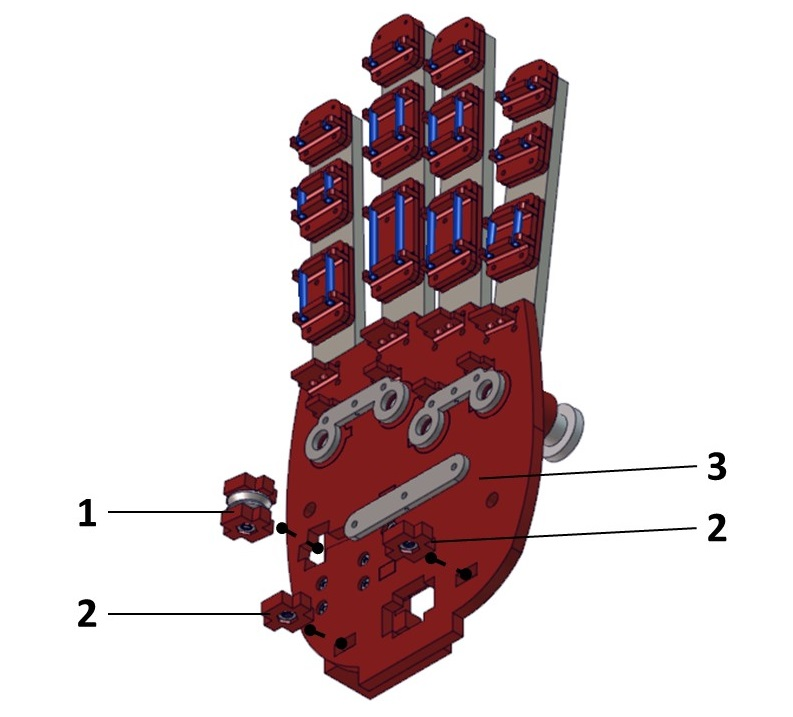
\includegraphics[trim={1cm, 0cm, 1cm, 0cm}, clip,scale = 0.35]{figures/Hand/palmTendonRouting_support.jpg}
    	\end{tabular}
	\end{minipage}
	\begin{minipage}[b]{0.4\linewidth}
	\begin{tabular}{ l l }
		{\circled{1}} & {Align part 1 with the}\\
		{} & {socket of part 2 as shown.} \\ \\
		{\circled{2}} & {Align part 3 with the}\\
		{} & {socket of part 2 as shown.} \\
    	\end{tabular}
  	\end{minipage}
};
\node[mytitle, right=10pt] at (box.north west) {Board 7.4.6: Attaching the Support of the Tendon Routing Base on the Palm};
\end{tikzpicture}%
\end{center}



\begin{table}[ht!]
	\centering
	\scalebox{0.9}{
		\begin{tabular}{ |c | c | c |}
			\hline
			\multicolumn{3}{|c|}{{\bf{Parts List 7.4.7}}} \\ \hline		
			{\bf{No}} & {\bf{Part Name}} & {\bf{Qty}}\\ \hline
			1 & palmDown & 1  \\ \hline
			2 & palmUp & 1  \\ \hline
			3 & M3X16 Socket Cup Screw & 1  \\ \hline
			4 & M3 Washer & 2  \\ \hline
			5 & M3 Nut & 1  \\ \hline
			6 & Plastic spacer 4mm & 1  \\ \hline	
			\multicolumn{3}{|c|}{{\bf{Tools}}} \\ \hline
			\multicolumn{3}{|c|}{{{Allen Wrench}}} \\ \hline		
		\end{tabular}
	}
\end{table}

\begin{center}
	\begin{tikzpicture}
	\node [mybox] (box){%
		\begin{minipage}[b]{0.50\linewidth}\centering
		\begin{tabular}{ l }
		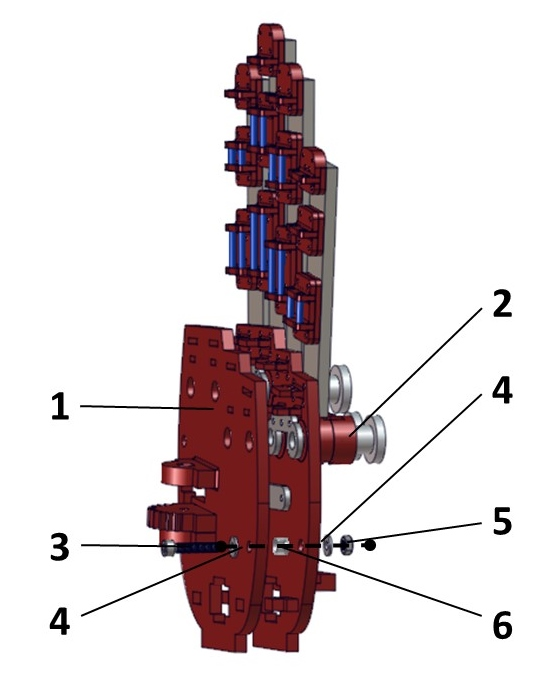
\includegraphics[trim={1cm, 0cm, 1cm, 0cm}, clip,scale = 0.5]{figures/Hand/palmUp_palmDown.jpg}
		\end{tabular}
		\end{minipage}
		\begin{minipage}[b]{0.4\linewidth}
		\begin{tabular}{ l l }
		{\circled{1}} & {Align palmUp with palmDown.} \\ \\
		{\circled{2}} & {Screw the M3X16 bolt through}\\
		{} &  {all fasteners as shown.} \\ \\
		{\circled{!}} & {The gap between palmUp and}\\
		{} & {palmDown parts should be 4mm.} \\
		\end{tabular}
		\end{minipage}
	};
	\node[mytitle, right=10pt] at (box.north west) {Board 7.4.7: Attaching the Upper and Lower Palm Parts};
	\end{tikzpicture}%
\end{center}

\newpage

\begin{table}[ht!]
	\centering
	\scalebox{0.97}{
		\begin{tabular}{ |c | c | c |}
			\hline
			\multicolumn{3}{|c|}{{\bf{Parts List 7.4.8}}} \\ \hline		
			{\bf{No}} & {\bf{Part Name}} & {\bf{Qty}}\\ \hline
			1 & M3 Nut & 4  \\ \hline
			2 & supportPulley1 part & 2  \\ \hline
			3 & Plastic Spacer 4mm & 4  \\ \hline
			4 & M3X18 Set Screw & 2  \\ \hline
			5 & V-Grooved Sealed Ball Bearing & 2  \\ \hline	
			\multicolumn{3}{|c|}{{\bf{Tools}}} \\ \hline
			\multicolumn{3}{|c|}{{{Screwdriver}}} \\ \hline		
		\end{tabular}
	}
\end{table}

\begin{center}
	\begin{tikzpicture}
	\node [mybox] (box){%
		\begin{minipage}[b]{0.50\linewidth}\centering
		\begin{tabular}{ l }
		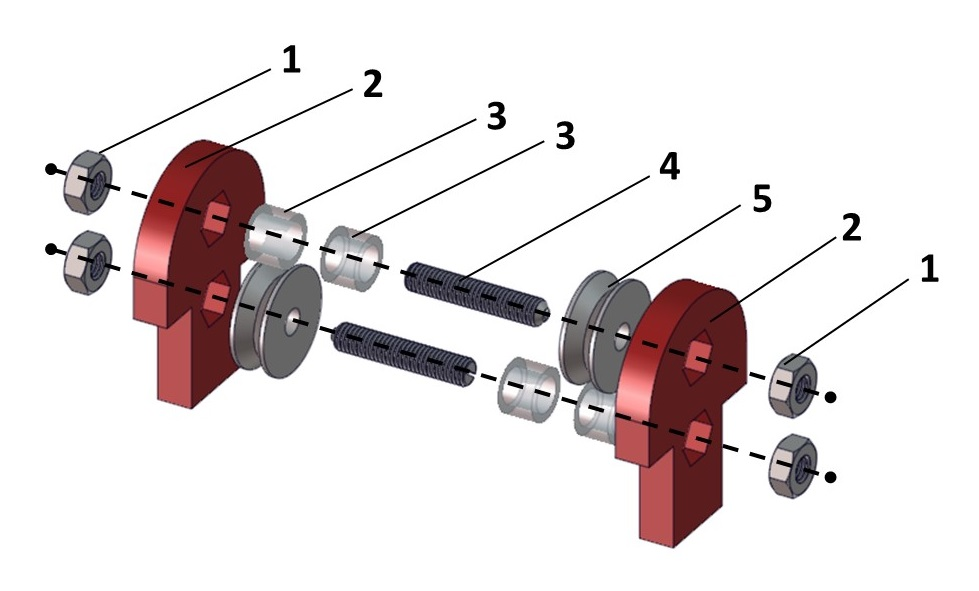
\includegraphics[trim={1cm, 0cm, 1cm, 0cm}, clip,scale = 0.3]{figures/Hand/tendonRoutingLast.jpg}
		\end{tabular}
		\end{minipage}
		\begin{minipage}[b]{0.5\linewidth}
		\begin{tabular}{ l l }
		{\circled{1}} & {Align the 4 M3 Nuts with}\\
		{} & {the sockets of supportPulley1.}\\ \\
		{\circled{2}} & {Align the 4 Spacers with}\\
		{} &  {the pulleys.} \\ \\
		{\circled{3}} & {Screw the M3X18 Set Screws}\\
		{} & {on all fasteners.} \\
		\end{tabular}
		\end{minipage}
	};
	\node[mytitle, right=10pt] at (box.north west) {7.4.8: Building the Tendon Routing Pulley Base II};
	\end{tikzpicture}%
\end{center}

\newpage

\subsection{Attaching the Thumb Locking Mechanism and Tendon Routing on the Palm}

\begin{table}[ht!]
	\centering
	\scalebox{0.97}{
		\begin{tabular}{ |c | c | c |}
			\hline
			\multicolumn{3}{|c|}{{\bf{Parts List 7.5.1}}} \\ \hline		
			{\bf{No}} & {\bf{Part Name}} & {\bf{Qty}}\\ \hline
			1 & Structure of Board 7.4.7 & 1  \\ \hline
			2 & Structure of Board 7.3.4 & 1  \\ \hline
			3 & M3X30 Set Screw & 1  \\ \hline
			4 & V-Grooved Sealed Ball Bearing & 1  \\ \hline
			5 & M3 Nut & 2  \\ \hline	
			\multicolumn{3}{|c|}{{\bf{Tools}}} \\ \hline
			\multicolumn{3}{|c|}{{{Screwdriver}}} \\ \hline		
		\end{tabular}
	}
\end{table}

\begin{center}
	\begin{tikzpicture}
	\node [mybox] (box){%
		\begin{minipage}[b]{0.50\linewidth}\centering
		\begin{tabular}{ l }
		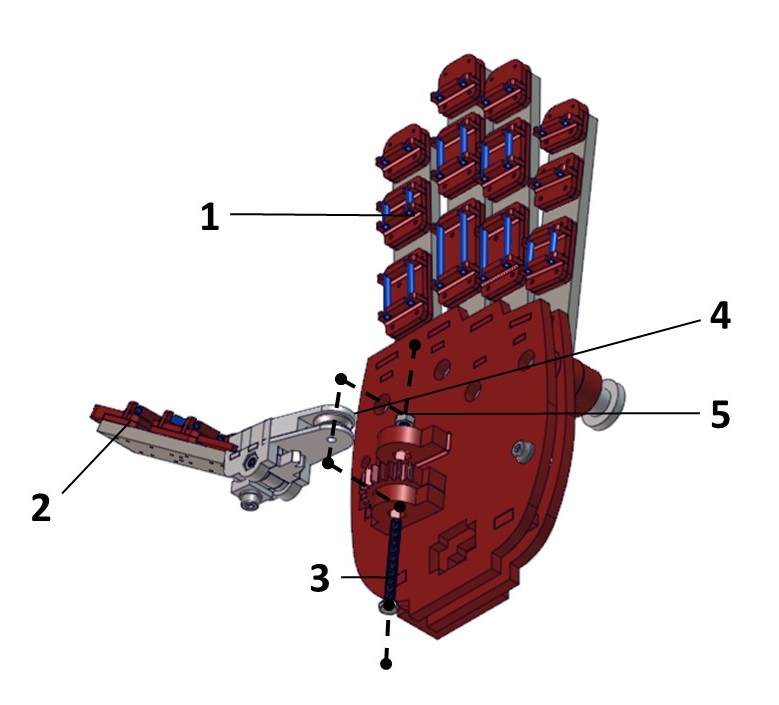
\includegraphics[trim={0cm, 0cm, 1cm, 0cm}, clip,scale = 0.37]{figures/Hand/palmUpPalmDown_thumb.jpg}
		\end{tabular}
		\end{minipage}
		\begin{minipage}[b]{0.4\linewidth}
		\begin{tabular}{ l l }
		{\circled{1}} & {Align the pulley to part 2.} \\ \\
		{\circled{2}} & {Align part 2 with part 1 as shown.} \\ \\
		{\circled{3}} & {Screw the M3X30 Set Screw}\\
		{} &  {on all fasteners.} \\
		\end{tabular}
		\end{minipage}
	};
	\node[mytitle, right=10pt] at (box.north west) {Board 7.5.1: Attaching the Thumb Locking Mechanism on its Palm Base};
	\end{tikzpicture}%
\end{center}


\begin{table}[ht!]
	\centering
	\scalebox{0.97}{
		\begin{tabular}{ |c | c | c |}
			\hline
			\multicolumn{3}{|c|}{{\bf{Parts List 7.5.2}}} \\ \hline		
			{\bf{No}} & {\bf{Part Name}} & {\bf{Qty}}\\ \hline
			1 & Structure of Board 7.5.1 & 1  \\ \hline
			2 & Structure of Board 7.4.8 & 1  \\ \hline		
		\end{tabular}
	}
\end{table}

\begin{center}
	\begin{tikzpicture}
	\node [mybox] (box){%
		\begin{minipage}[b]{0.5\linewidth}\centering
		\begin{tabular}{ c }
		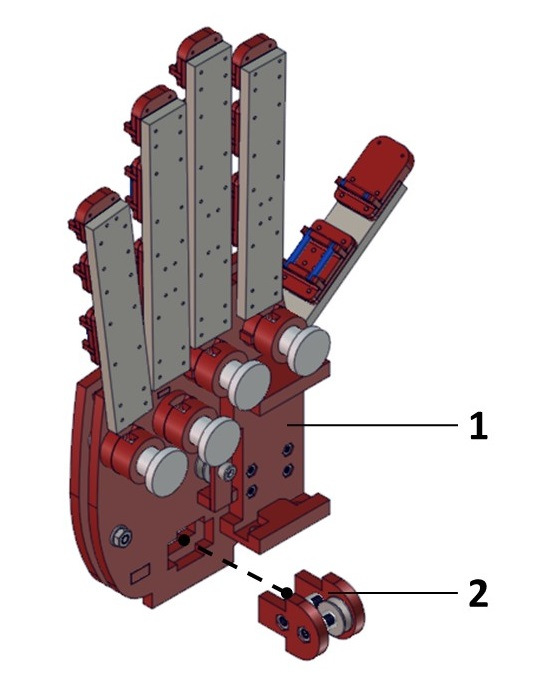
\includegraphics[trim={1cm, 0cm, 1cm, 0cm}, clip,scale = 0.5]{figures/Hand/palmUpPalmDownThumb_tendonRouting.jpg}
		\end{tabular}
		\end{minipage}
		\begin{minipage}[b]{0.5\linewidth}
		\begin{tabular}{ l l }
		{\circled{1}} & {Attach part 2 on part 1.} \\
		\end{tabular}
		\end{minipage}
	};
	\node[mytitle, right=10pt] at (box.north west) {Board 7.5.2: Attaching the Thumb Tendon Routing Base on the Palm};
	\end{tikzpicture}%
\end{center}


\begin{table}[ht!]
	\centering
	\scalebox{0.97}{
		\begin{tabular}{ |c | c | c |}
			\hline
			\multicolumn{3}{|c|}{{\bf{Parts List 7.5.3}}} \\ \hline		
			{\bf{No}} & {\bf{Part Name}} & {\bf{Qty}}\\ \hline
			1 & Dyneema & --  \\ \hline
			2 &  V-Grooved Sealed Ball Bearing & 2  \\ \hline
			\multicolumn{3}{|c|}{{\bf{Tools}}} \\ \hline
			\multicolumn{3}{|c|}{{{Long Needles}}} \\ \hline		
		\end{tabular}
	}
\end{table}

\begin{center}
	\begin{tikzpicture}
	\node [mybox] (box){%
		\begin{minipage}[b]{0.50\linewidth}\centering
		\begin{tabular}{ c }
		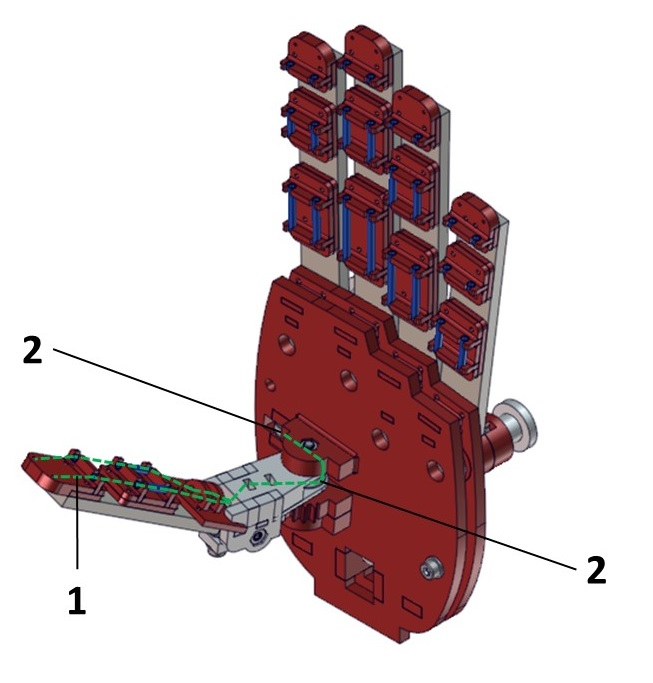
\includegraphics[trim={0cm, 0cm, 1cm, 0cm}, clip,scale = 0.45]{figures/Hand/palmUpPalmDownThumbTendonRoutingRoute1.jpg}
		\end{tabular}
		\end{minipage}
		\begin{minipage}[b]{0.4\linewidth}
		\begin{tabular}{ l l }
		{\circled{1}} & {Pass the thumb tendon around}\\
		{} & {pulley-part 2.} \\ \\
		{\circled{!}} & {Long needles can be used}\\
		{} & {to simplify the process.} \\
		\end{tabular}
		\end{minipage}
	};
	\node[mytitle, right=10pt] at (box.north west) {Board 7.5.3: Passing the thumb Tendon around Tendon Routing Pulley 1};
	\end{tikzpicture}%
\end{center}

\newpage

\begin{table}[ht!]
	\centering
	\scalebox{0.97}{
		\begin{tabular}{ |c | c | c |}
			\hline
			\multicolumn{3}{|c|}{{\bf{Parts List 7.5.4}}} \\ \hline		
			{\bf{No}} & {\bf{Part Name}} & {\bf{Qty}}\\ \hline
			1 & Dyneema & --  \\ \hline
			2 &  V-Grooved Sealed Ball Bearing & 2  \\ \hline
			\multicolumn{3}{|c|}{{\bf{Tools}}} \\ \hline
			\multicolumn{3}{|c|}{{{Long Needles}}} \\ \hline		
		\end{tabular}
	}
\end{table}

\begin{center}
	\begin{tikzpicture}
	\node [mybox] (box){%
		\begin{minipage}[b]{0.50\linewidth}\centering
		\begin{tabular}{ l }
		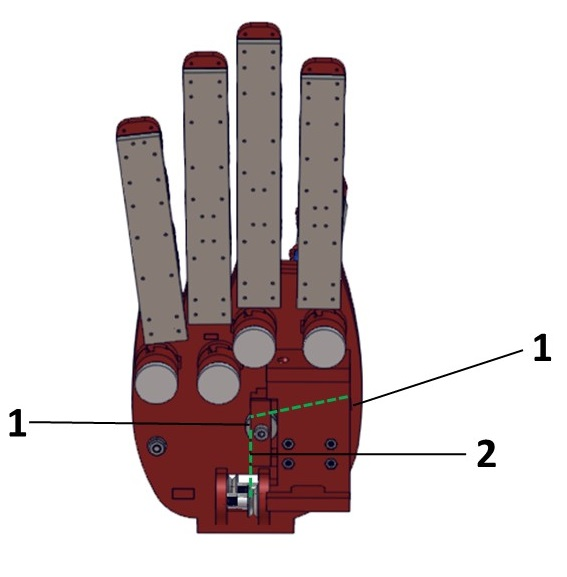
\includegraphics[width = 10cm]{figures/Hand/palmUpPalmDownThumbTendonRoutingRoute2.jpg}
		\end{tabular}
		\end{minipage}
		\begin{minipage}[b]{0.4\linewidth}
		\begin{tabular}{ l l }
		{\circled{1}} & {Pass the thumb tendon around}\\
		{} & {pulley-part 2.} \\ \\
		{\circled{!}} & {Long needles can be used}\\
		{} & {to simplify the process.} \\	\\ \\ \\
		\end{tabular}
		\end{minipage}
	};
	\node[mytitle, right=10pt] at (box.north west) {Board 7.5.4: Passing the thumb Tendon around Tendon Routing Pulley 2};
	\end{tikzpicture}%
\end{center}

\newpage

\subsection{Attaching the Base Flange on the Hand}

\begin{table}[ht!]
	\centering
	\scalebox{0.97}{
		\begin{tabular}{ |c | c | c |}
			\hline
			\multicolumn{3}{|c|}{{\bf{Parts List 7.6.1}}} \\ \hline		
			{\bf{No}} & {\bf{Part Name}} & {\bf{Qty}}\\ \hline
			1 & Prosthetic Hand & 1  \\ \hline
			2 &  flangePlate part & 1  \\ \hline
			3 &  M3X20 Socket Cup Screw & 2  \\ \hline
			4 &  dovetailFemale part & 1  \\ \hline
			\multicolumn{3}{|c|}{{\bf{Tools}}} \\ \hline
			\multicolumn{3}{|c|}{{{Allen Wrench}}} \\ \hline	
			\multicolumn{3}{|c|}{{{ABS Glue}}} \\ \hline	
		\end{tabular}
	}
\end{table}

\begin{center}
	\begin{tikzpicture}
	\node [mybox] (box){%
		\begin{minipage}[b]{0.5\linewidth}\centering
		\begin{tabular}{ l }
		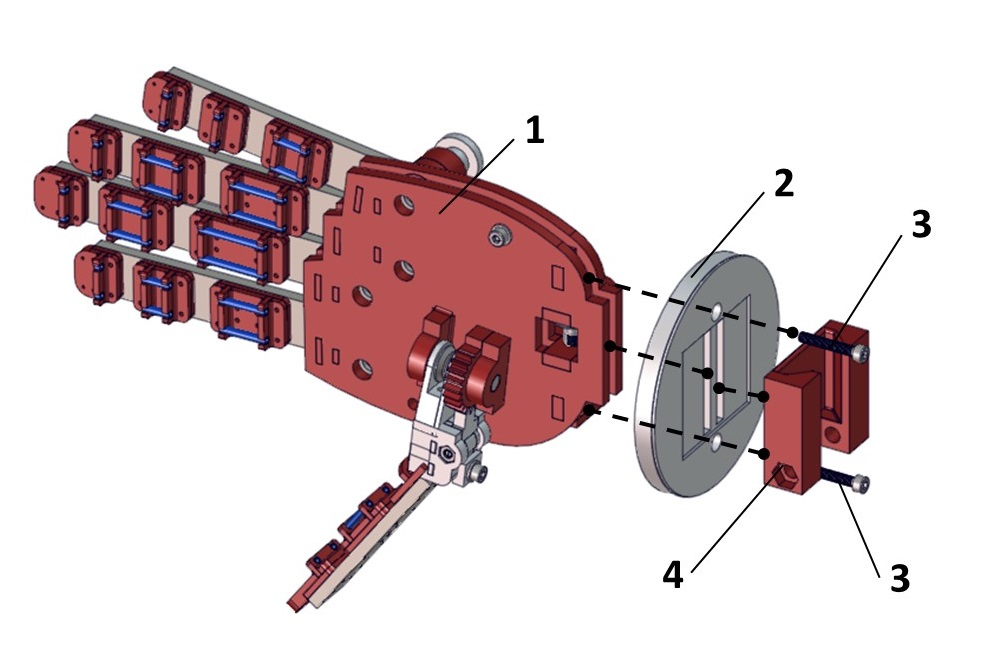
\includegraphics[trim={1cm, 0cm, 1cm, 0cm}, clip,scale = 0.3]{figures/Hand/palmUpPalmDownThumb_flange.jpg}
		\end{tabular}
		\end{minipage}
		\begin{minipage}[b]{0.37\linewidth}
		\begin{tabular}{ l l }
		{\circled{1}} & {Glue the flangePlate}\\
		{} & {on the dovetailFemale.} \\ \\
		{\circled{2}} & {Place the flangePlate}\\
		{} & {on the Hand.} \\ \\
		{\circled{3}} & {Screw M3X20 bolts through}\\
		{} & {the M3 Nuts of the Hand.} \\
		\end{tabular}
		\end{minipage}
	};
	\node[mytitle, right=10pt] at (box.north west) {Board 7.6.1: Attaching the Base Flange on the Hand Palm};
	\end{tikzpicture}%
\end{center}

\subsection{Hand is Assembled}

{\large Congratulations you have created an affordable, anthropomorphic, personalized, light-weight prosthetic hand!}

\begin{center}
   \fbox{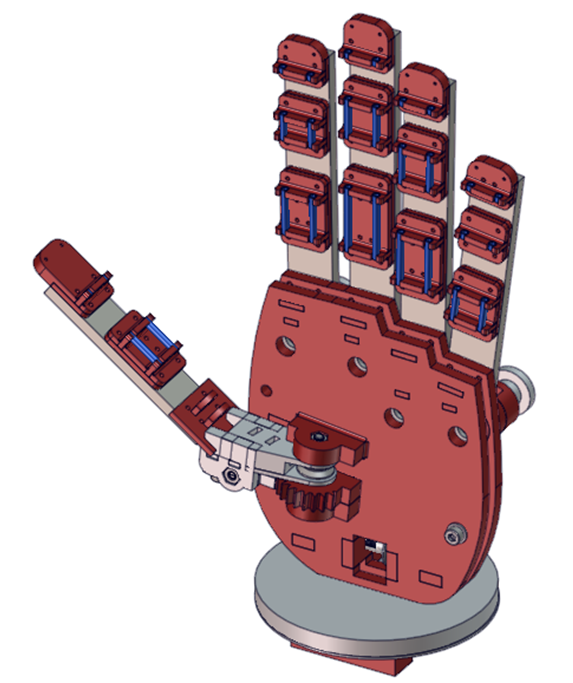
\includegraphics[width=7cm]{figures/AnthropomorphicHandAssembly_Guide.png}}
\end{center} 
		